% !TeX root = Protokoll.tex
 \begin{figure}[h!]
 	\centering
 	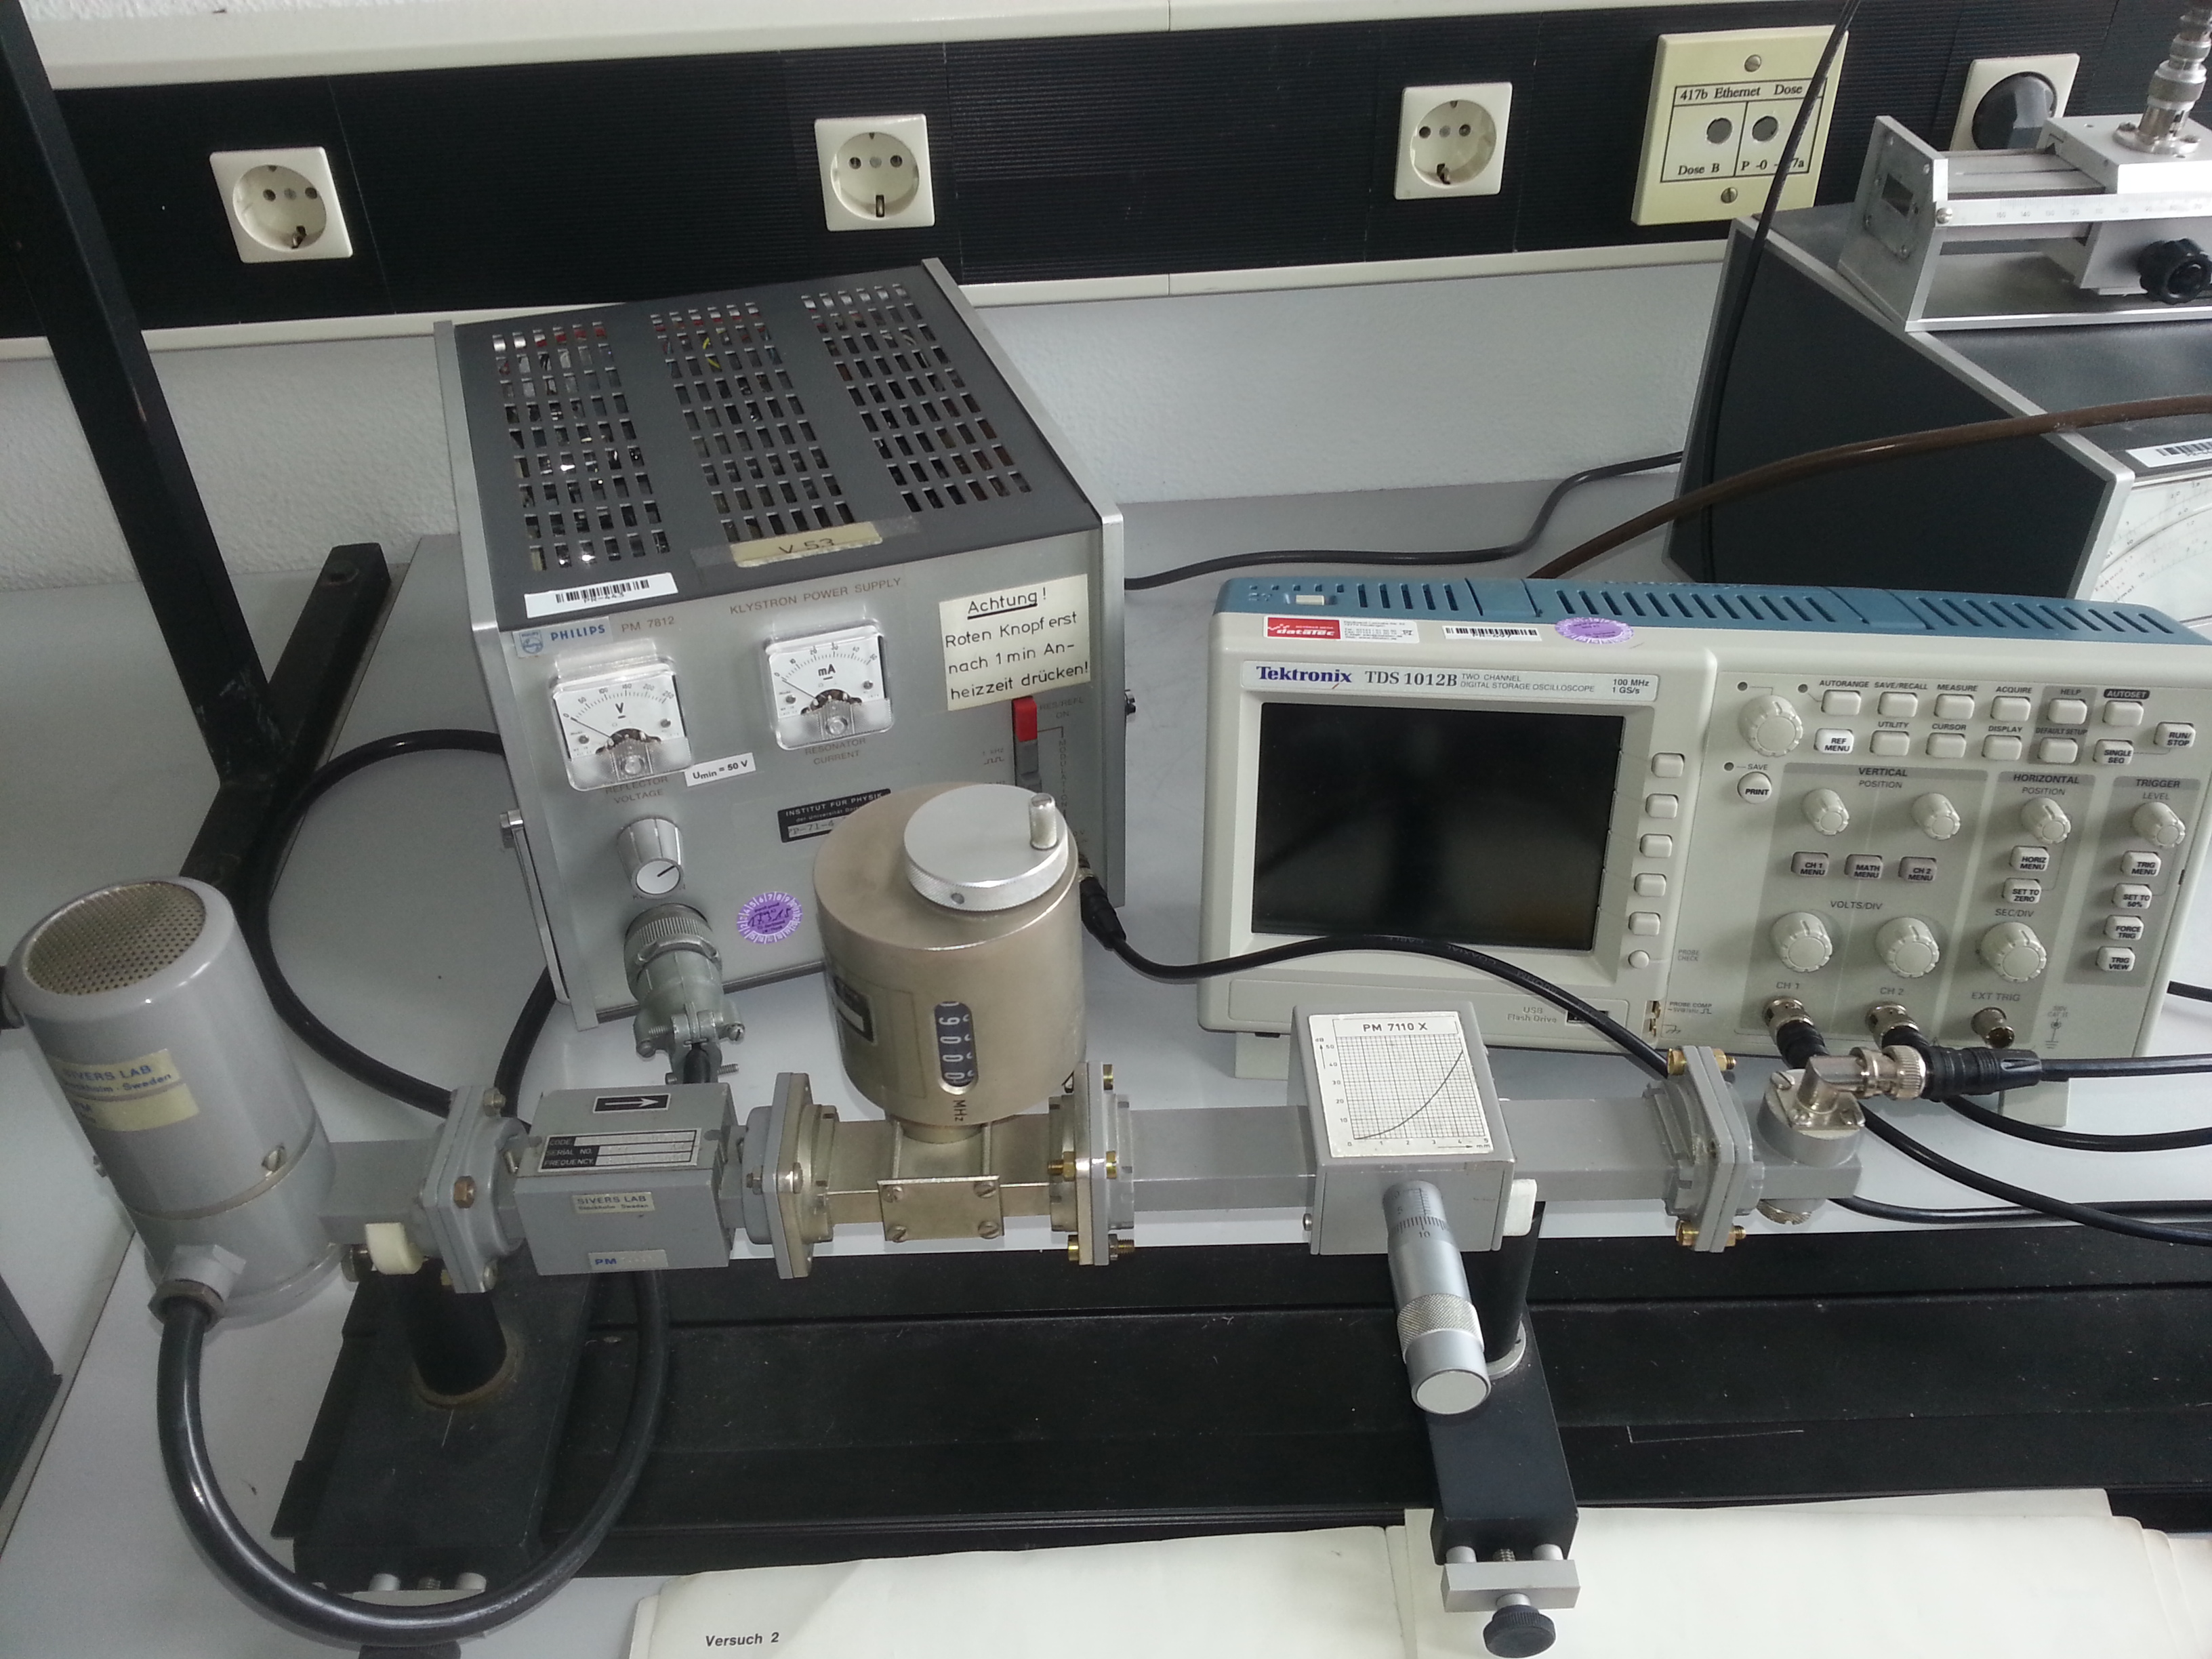
\includegraphics[scale = 0.1]{../Grafiken/Aufbau_1.jpg}
 	\caption{Der Aufbau zur vermessung der Moden mithilfe eines Oszilloskops\label{fig:Moden}}
 \end{figure}
 Als erstes werden die Moden des Klystron Vermessen. Dazu wird der Aufbau aus \cref{fig:Moden} verwendet. Ganz links ist das Klystron zu sehen. Rechts davon im Hintergrund ist die Spannungsquelle für das Klystron. Davor ist der Frequenzmesser zusehen, an dem die Frequenz des Klystrons eingestellt werden kann. Rechts davon ist das Dämpfungsglied zu sehen. Am ende des Hohlleiters ist der Detektor angebracht mit das Oszilloskop angeschlossen wird, das Oszilloskop ist hinter dem Hohlleiter rechts zu sehen. Am zweiten Channel des Oszilloskops ist die Spannungsquelle des Klystrons angebracht. Dadurch kann die Angelegte Spannung gegen die Spannung am ende des Hohlleiters angezeigt werden. Das Dämpfungsglied wird auf 30dB gestellt. Durch Verstellen der Reflektorspannung, können verschiedene Moden erzeugt werden. Eine Mode ist in \cref{fig:BeispielMode} zusehen. Durch verstellen der Frequenz kann eine Delle (dip) in der Mode erzeugt werden.
 \begin{figure}[h!]
  	\centering
  	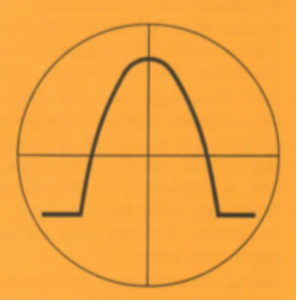
\includegraphics[scale = 1]{../Grafiken/Moden.pdf}
  	\caption{Beispiel einer Mode, wie sie auf dem Oszilloskops dargestellt wird.\cite{V53}\label{fig:BeispielMode}}
  \end{figure}
Der dip wird solange bewegt bis er an der Spitze der Mode ist und die dazugehörige Frequenz $f_0$ wird gemessen. Danach wird die Frequenz auf \SI{9}{\giga\hertz} eingestellt. Die Spannung für das Klystron wird verstellt bis sie ein mal der Anfang und das Ende der Mode auf der Mittellinie war, sowie einmal das Maximum. Die Eingestellten Spannungen werden gemessen. Dies wird für drei Moden wiederholt.\\
Es wird nun die höchste Mode für eine Frequenz von \SI{9}{\giga\hertz} eingestellt. Die Frequenz wird so eingestellt das die Delle beim Maximum ist. Die Spannung wird so eingestellt das der dip auf der Mittellinie ist. Frequenz und Spannung werden notiert. Anschließend wird die Delle so verschoben das sie auf halber Höhe links vom Maximum ist und die Spannung wird so angepasst, dass die Delle wieder auf der Mittellinie ist. Frequenz und Spannung wird gemessen. Diese Messung wird noch mal für die rechte Seite wiederholt.
\subsection{Frequenz Messung}
\begin{figure}[h!]
	\centering
	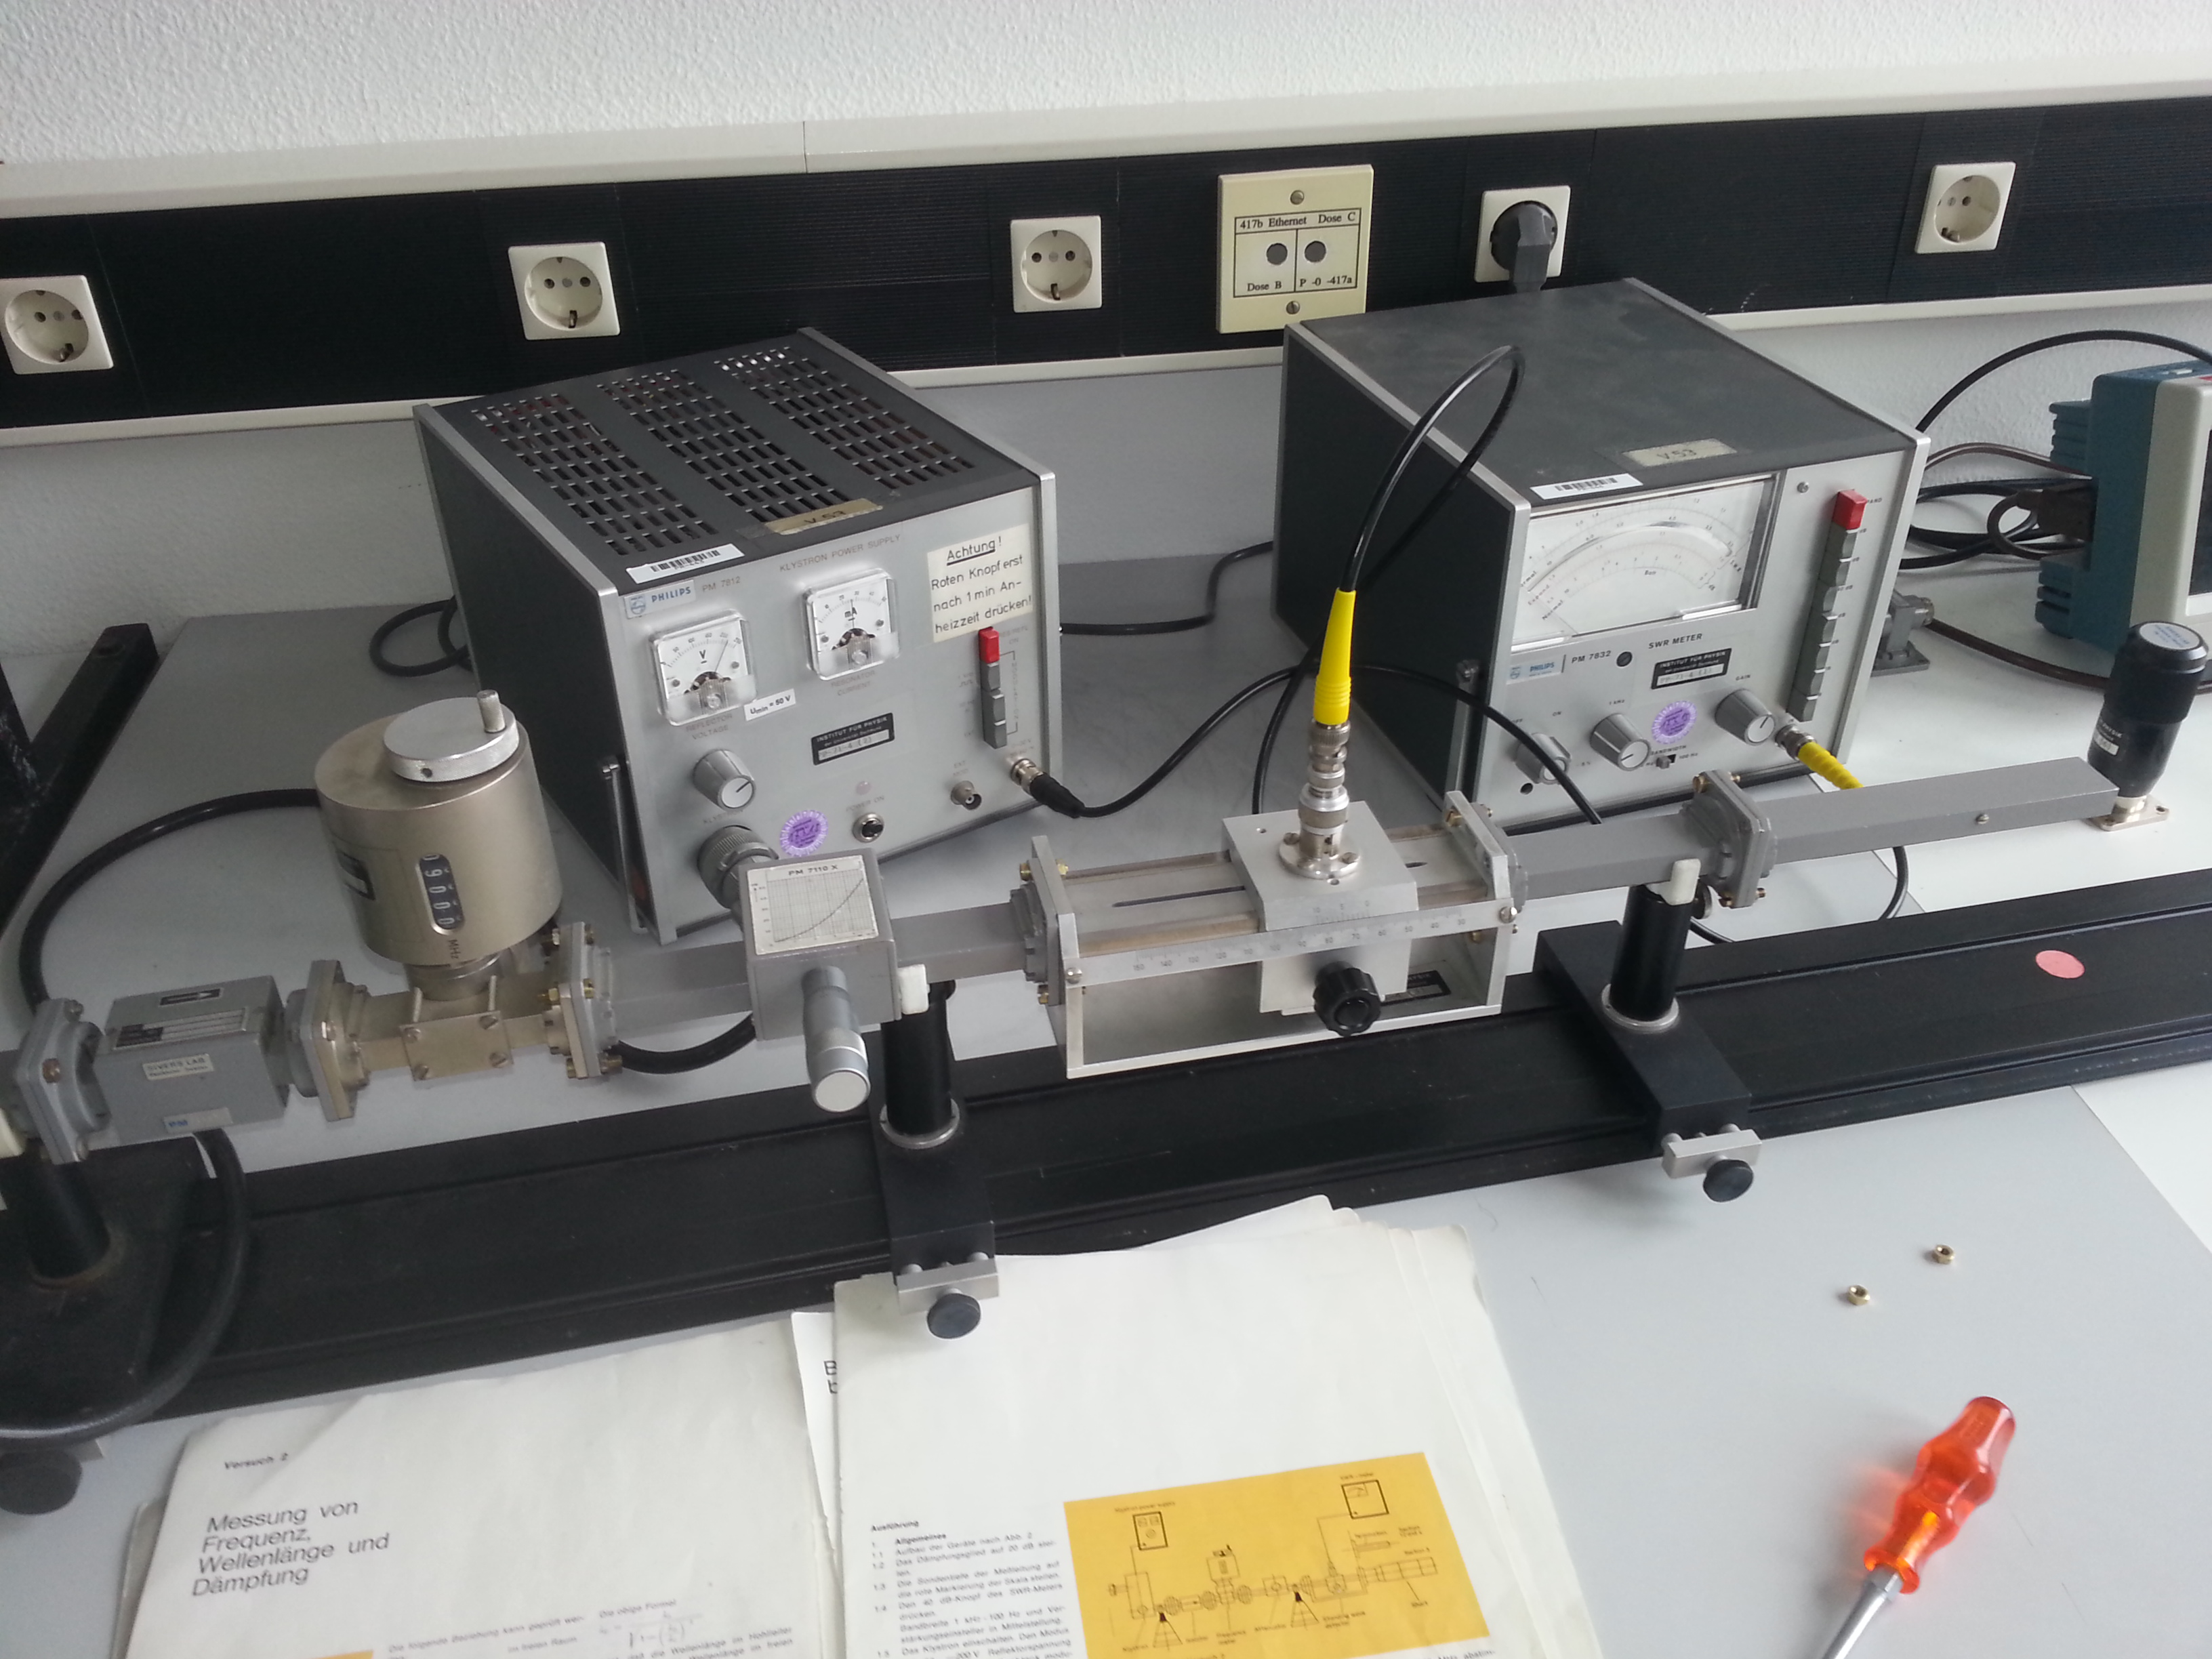
\includegraphics[scale = 0.1]{../Grafiken/Aufbau_2.jpg}
	\caption{Aufbau zur Vermessung der Frequenz der Mikrowellen.}\label{fig:AufbauFrequenz}
\end{figure}
Anstelle des Detektors wird eine Sonde verwendet. Die Sonde ist auf einer Schiene und kann damit entlang des Hohlleiters bewegt werden, zu dem kann die Höhe der Sonde verstellt werden. Mithilfe der Sonde wird ein SWR-Meter angeschlossen. Am Ende des Hohlleiters befindet sich ein Abschluss. Der Aufbau ist in \cref{fig:AufbauFrequenz} zu sehen und das Dämpfungsglied wird auf 20 dB gestellt. Die Reflektorspannung so an Passen das ein Maximum auf dem SWR-Meter zusehen ist. Danach wird der Frequenzmesser so lange gedreht bis ein Rückgang am SWR-Meter zu sehen ist. Die Frequenz wird auf ein Minimum des SWR-Meters eingestellt und notiert.\newpage
\subsection{Wellenlängen Messung}\label{sec:Wellenlänge}
\begin{figure}[h!]
	\centering
	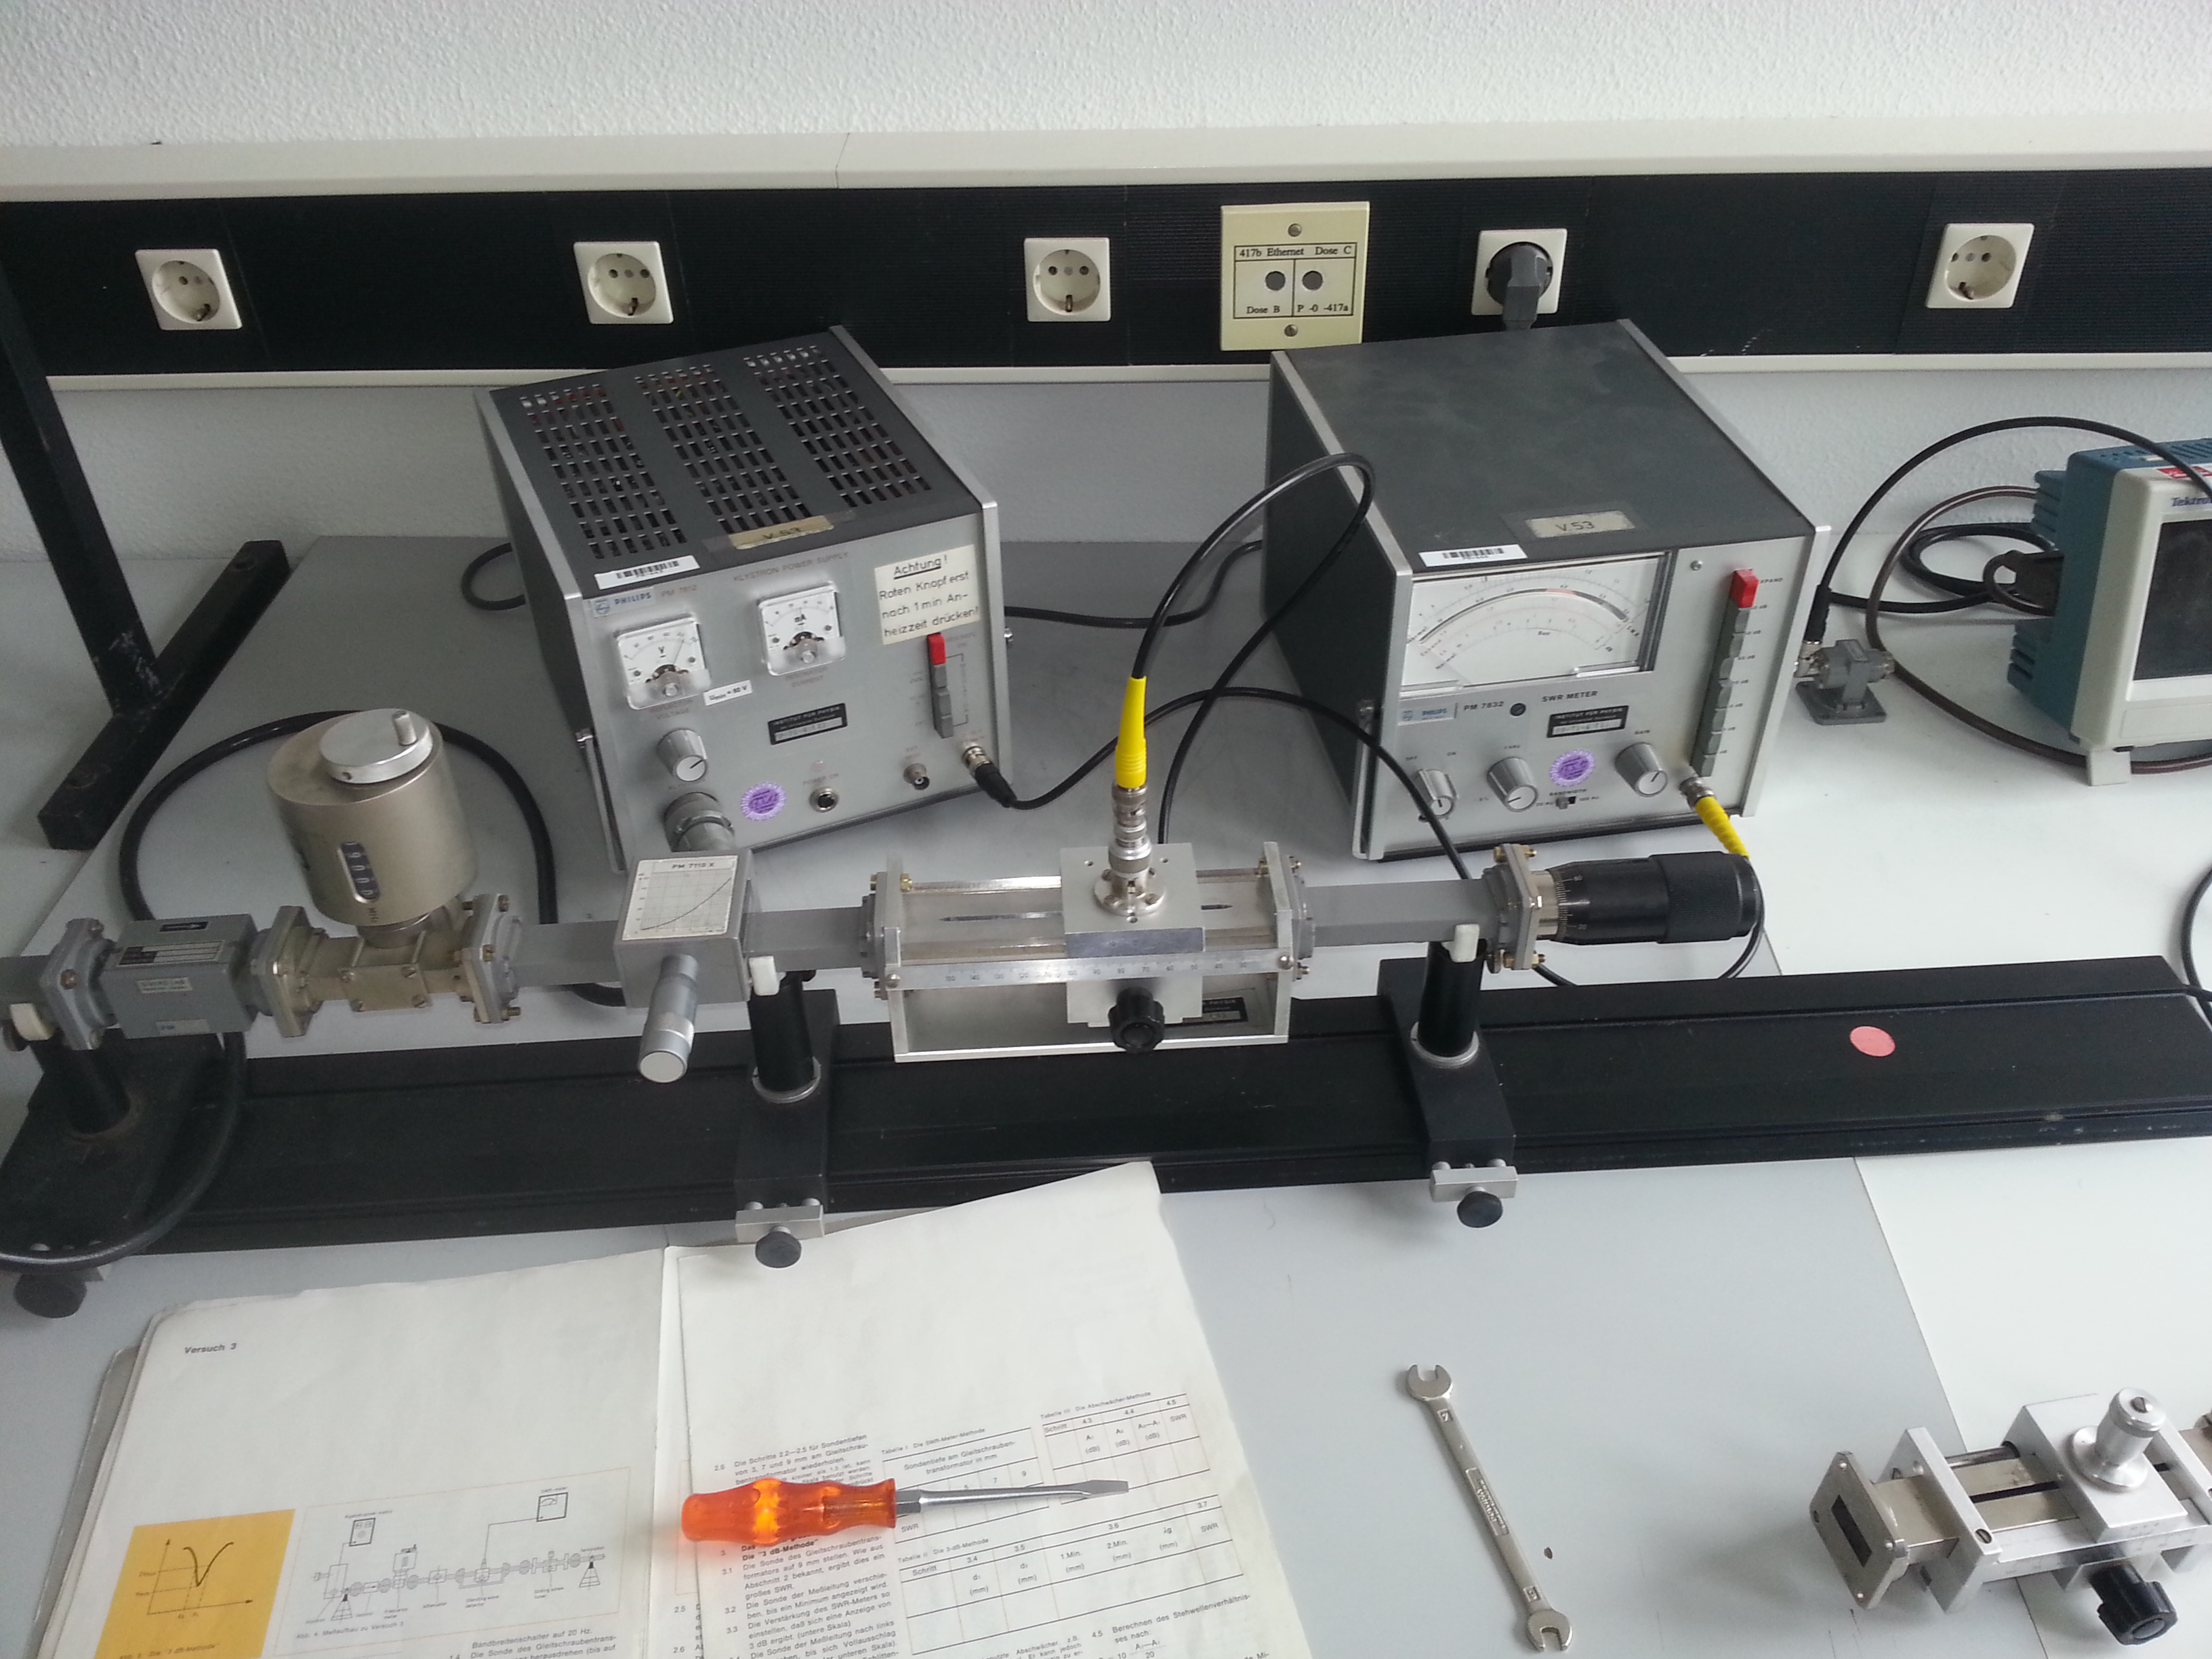
\includegraphics[scale = 0.1]{../Grafiken/Aufbau_3.jpg}
	\caption{Aufbau zur Vermessung der Wellenlänge der Mikrowellen.}\label{fig:AufbauWellenlänge}
\end{figure}
Zur Vermessung der Wellenlänge wird der Aufbau nach \cref{fig:AufbauWellenlänge} verwendet. Dabei wurde der Abschluss durch ein einstellbaren Defekt aus getauscht. Durch das verschieben der Sonde wird nun die Positionen von zwei auf einander folgenden Minima gemessen. Zusätzlich wird die Länge der größeren kante notiert.
\subsection{Dämpfungsmessung}
Es wird der Aufbau aus der Frequenzmessung verwendet (\cref{fig:AufbauFrequenz}). Das SWR-Meter wird so eingestellt, dass auf der unteren Skala die Dämpfung auf \SI{0}{\deci\bel} steht. Nun wird das Dämpfungsglied verstellt, so das der Zeiger auf \SI{2}{\deci\bel} steht und die eingestellte Dämpfung notiert. Dies wird für  \SI{2}{\deci\bel} schritte bis \SI{10}{\deci\bel}. Dabei wird an dem Dämpfungsglied ein Abstand in \SI{}{\milli\meter} eingestellt, allerdings kann dies durch einen Graphen auf dem Dämpfungsglied in \SI{}{\deci\bel} umgerechnet werden.
 \newpage
\subsection{Kleine und mittlere Welligkeitsmessung}
\begin{figure}[h!]
	\centering
	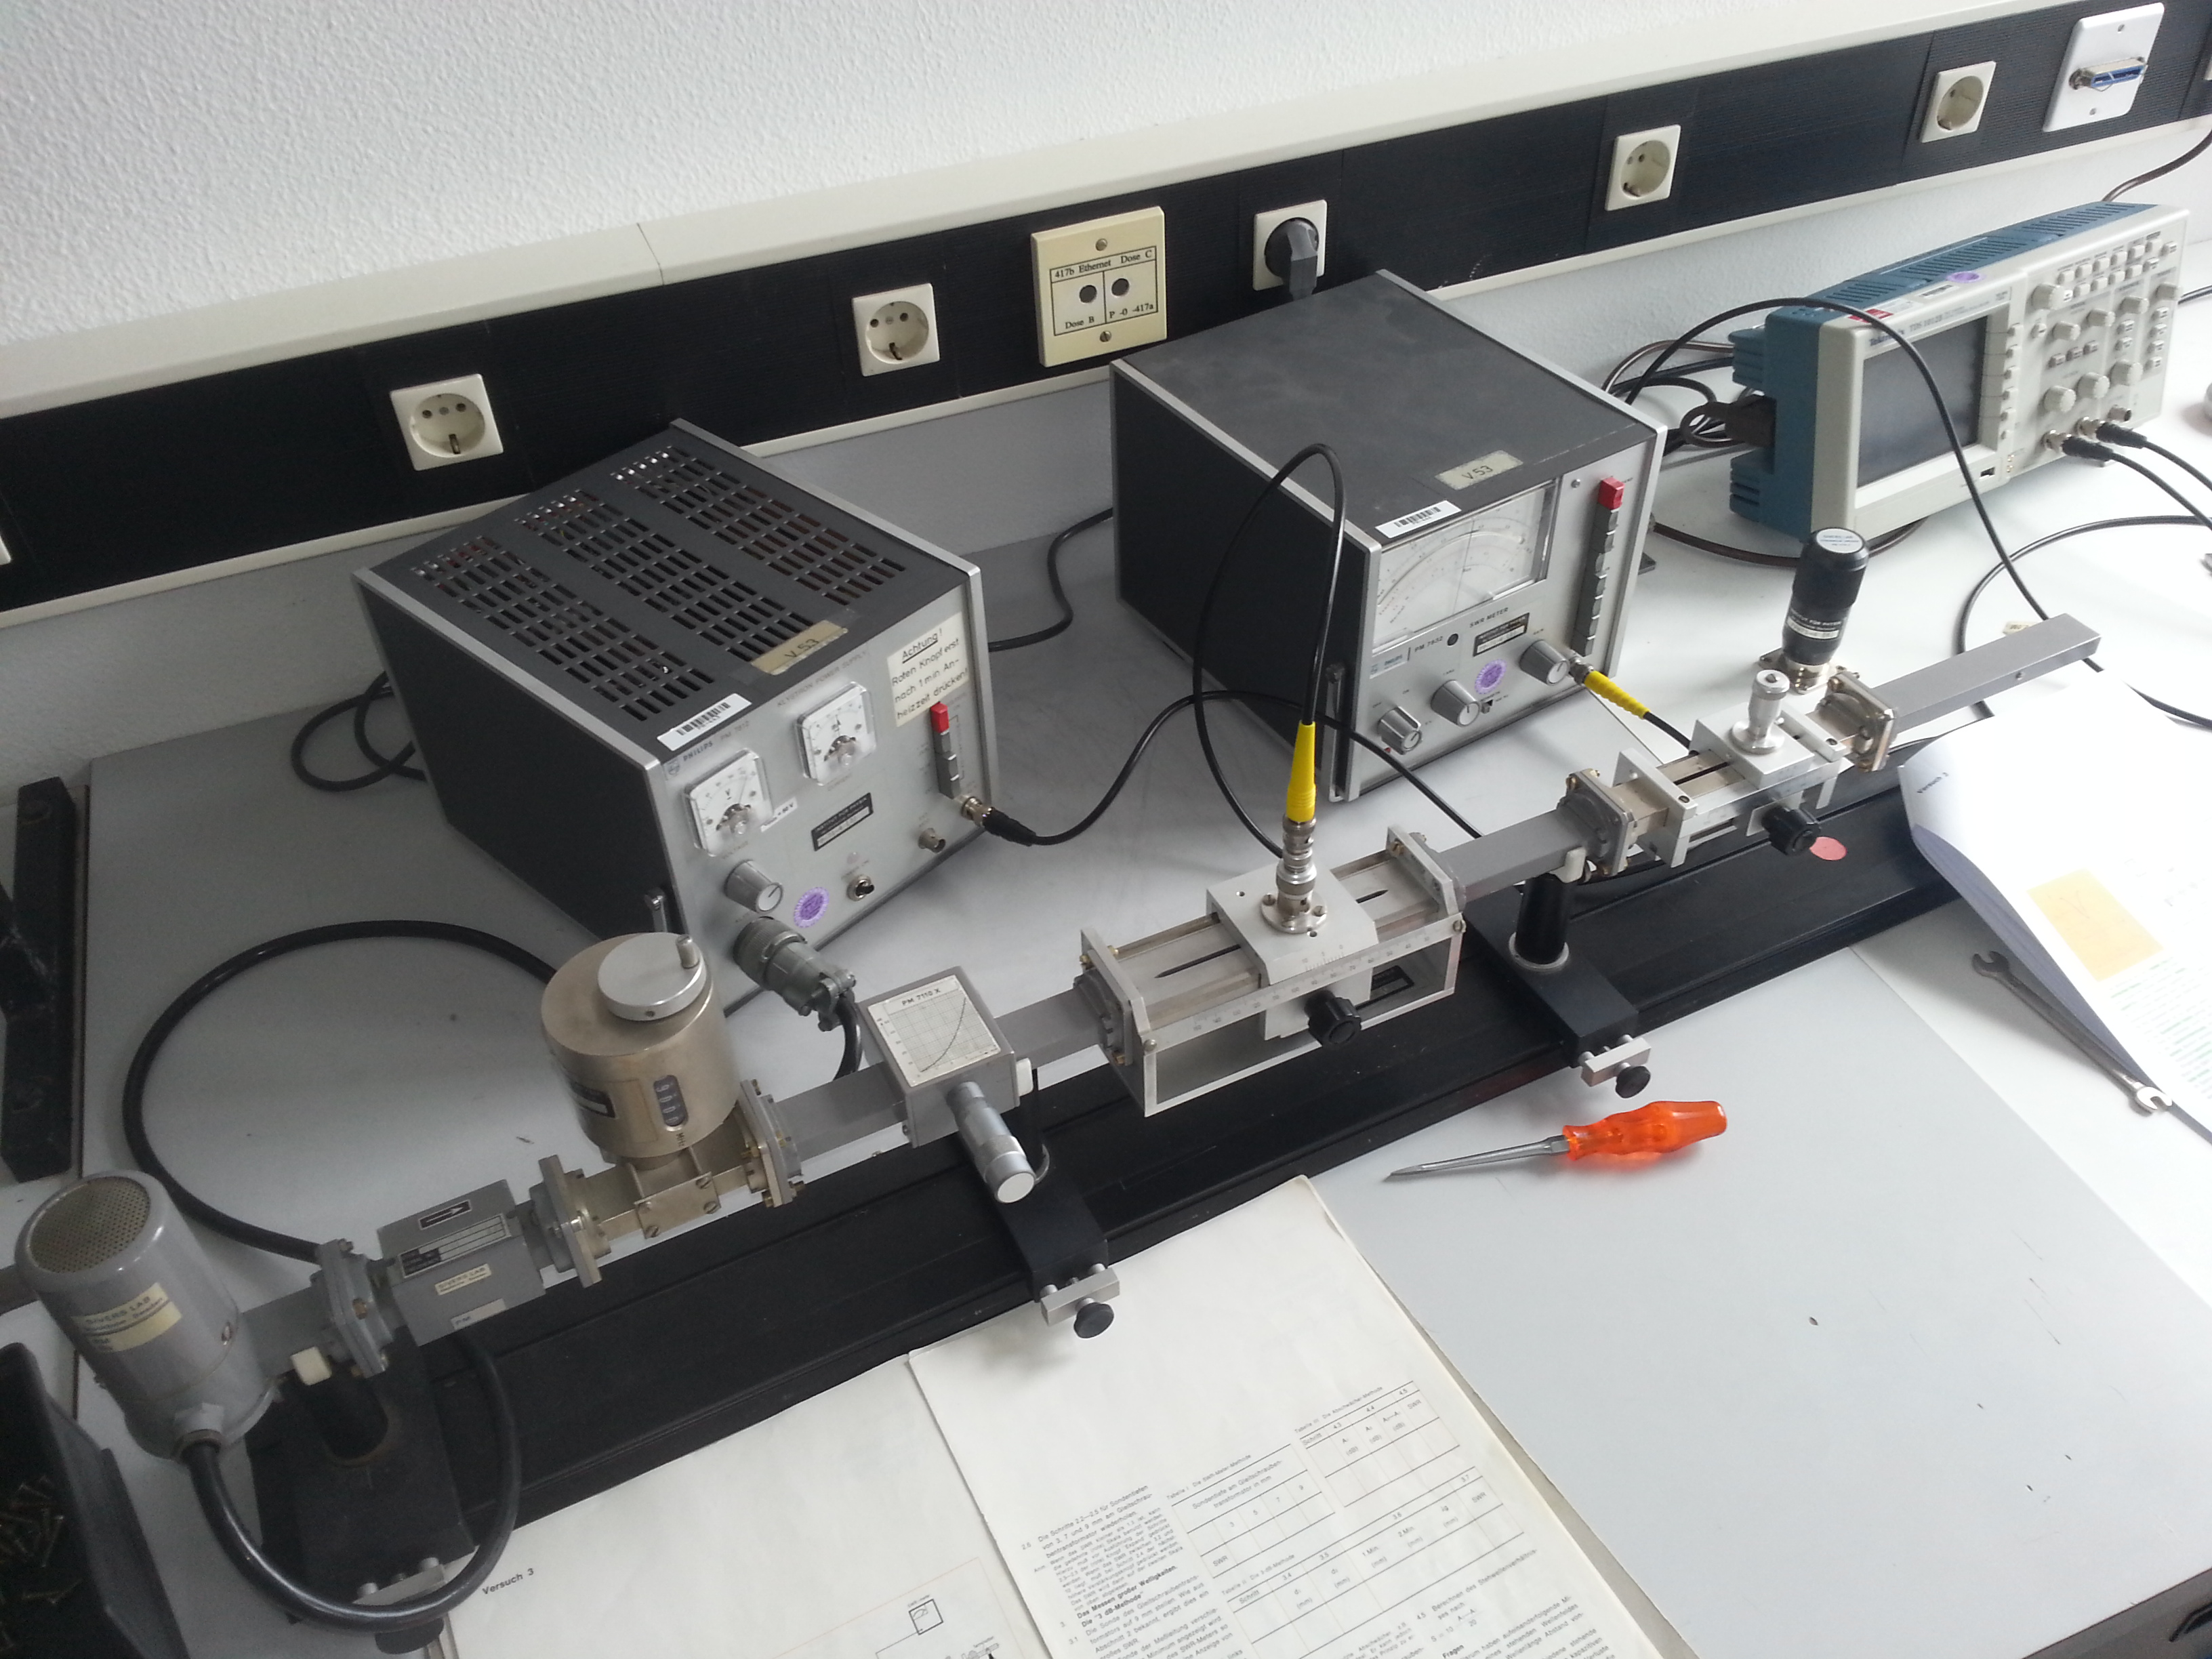
\includegraphics[scale =0.1]{../Grafiken/Aufbau_5.jpg}
	\caption{Der Verwendete auf Bau für die kleine und mittlere Welligkeitsmessung\label{fig:AufbauWellig}}
\end{figure}
Zwischen dem Abschluss und der Halterung für die Diode wird ein Gleitschraubentransformator eingebaut, wobei der Kopf raus gedreht ist. Das Dämpfungsglied wird auf \SI{20}{\deci\bel} eingestellt und die Frequenz wird auf \SI{9}{\giga\hertz} eingestellt. Der Ausschlag des SWR-Meters sollte im Mittelbereich liegen. Den Kopf auf \SI{5}{\milli\meter} heraus drehen. Die Sonde verschieben bis auf dem SWR-Meter ein Maximum zu erkennen ist. Dann das SWR-Meter so verstellen das es 1,0SWR anzeigt. Dann wird die Sonde Verschoben das ein Minimum erkennbar ist, der SWR-Wert wird gemessen. Dies wird für die Tiefen von \SI{3}{\milli\meter}, \SI{7}{\milli\meter} und \SI{9}{\milli\meter} wiederholt.
\subsection{Vermessung der großen Welligkeit}
\subsubsection{Die 3dB-Methode}
Die große Welligkeit wird mithilfe der \SI{3}{\deci\bel}-Methode vermessen. Die Tiefe bleibt bei \SI{9}{\milli\meter}. Die Sonde wird in ein Minimum verschoben. Das SWR-Meter wird so eingestellt das es \SI{3}{\deci\bel} anzeigt. Die Sonde wird nach ein mal nach links und ein mal nach rechts verschoben, bis zum Vollausschlag. die beiden Positionen werden notiert. Wie in \cref{sec:Wellenlänge} erklärt wird die Wellenlänge gemessen. Der SWR-Wert lässt sich durch 
\begin{align}
	S=\sqrt{1+\frac{1}{\sin\frac{\pi ( d_\text{l} - d_\text{r} ) }{ \lambda_g }}} \approx \frac{ \lambda_g }{\pi(d_\text{l} - d_\text{r})}
\end{align}
berechnen.
\subsubsection{Die Abschwächer-Methode}
Die große Welligkeit wird ebenfalls mit der Abschwächer-Methode gemessen.Der Versuch wird nach \cref{fig:AufbauWellig} aufgebaut. Das Gleitschraubentransformator wird auf \SI{9}{\milli\meter} Tiefe gestellt.
Die Sonde verschieben bis ein Minimum erkennbar ist. Das Dämpfungsglied auf \SI{20}{\deci\bel} einstellen und SWR-Meter so verstellen das es auf \SI{3}{\deci\bel} steht. Die Sonde wird nun auf der Schiene bewegt und mithilfe des Dämpfungsglieds wird, die Anzeige des SWR-Meters im Bereich gehalten. Auf diese weise wird die Sonde in ein Maximum verschoben, anschließend wird mit dem Dämpfungsglied das SWR-Meter auf \SI{3}{\deci\bel} eingestellt. Es wird der Anfangswert des Dämpfungsglieds und der Endwert gemessen. Daraus lässt sich die Welligkeit mithilfe von 
\begin{align}
	S=10\frac{A_2-A_1}{20}
\end{align}
bstimmen.